\section{Formalization}
\label{sec:Formalization}
In this chapter we define the terms suggestion and applicable suggestion. We introduce possible ways to refine a suggestion and to add domain specific knowledge.

\begin{figure}
    \centering
    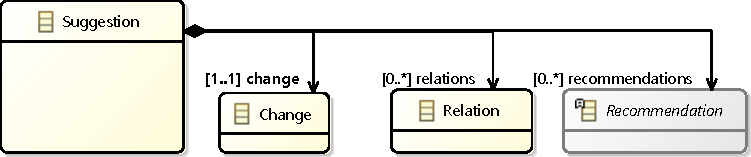
\includegraphics[width=\columnwidth]{images/Suggestion.pdf}
    \caption{A \textsf{Suggestion} holds for a single \textsf{Change} linked to elements in a View Type through \textsf{Relation}s, and consists of a set of \textsf{Recommendation}s.}
    \label{fig:Suggestion}
\end{figure}

\begin{figure}
    \centering
    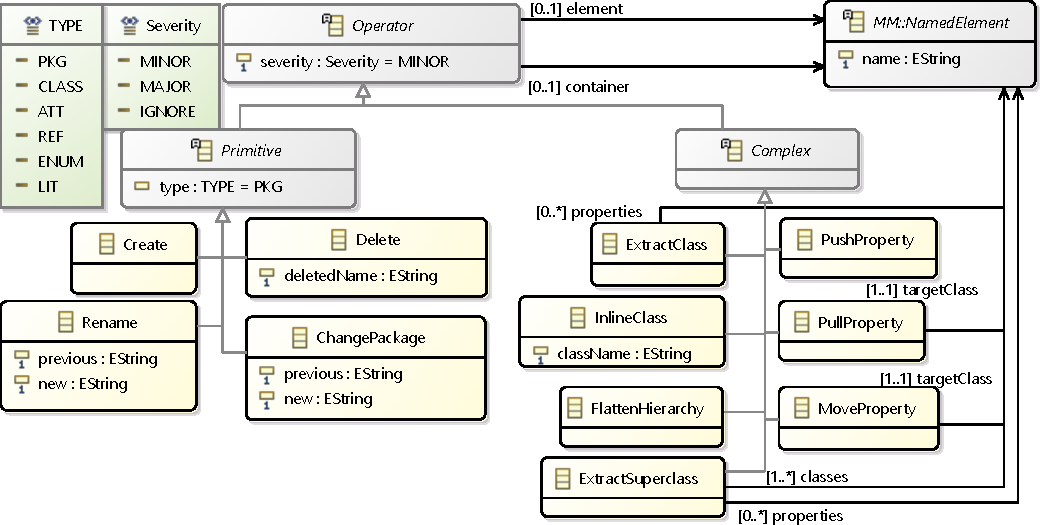
\includegraphics[width=\columnwidth]{Change.pdf}
    \caption{Possible \textsf{Change}s operated on a \metamodel \MA{This really corresponds to the \textsf{Opeartor} column of Table \ref{tab:suggestions}, where \textsf{ApplicationPattern} maps the column \textsf{Condition to offer...}.}}
    \label{fig:Change}
\end{figure}


\begin{definition}[Suggestion]\label{def:suggestion}
We define a suggestion $SUG$ as a 4-Tuple of a type of a change on the \metamodel $MMC$, a view generation transformation $VGT$ (which link to the \metamodel and the \viewtype),  constraints $CON$ and a suggestion content $SUC$. Short: $SUG = (MMC, VGT, CON, SUC)$
\end{definition}
Possible $MMC$ are defined in \cref{tab:suggestions}. A suggestion always contains one change. Change sequences that have domain semantics should define a new complex change, because the contained domain knowledge is interesting for other analyses besides suggestions. The view generation operators $VGO$ are defined in \cref{fig:model-query-operators}. They can be combined to a $VGT$. $VGTs$ may form a hierarchy that can be used for the refinement of suggestions. The constraints are defined on either the \metamodel, its instance, the view generation operators or the target \metamodel. Constraints may also form a hierarchy for the refinement of suggestions. The $SUC$ is either a textual description of the suggestion or a formalisation of possible changes or a change on the \viewtype or a combination of all three. Either the textual description or the formalisation and the possible changes are preferable as it enables the methodologist to precisely define the change on the \viewtype \metamodel as well as giving some rationale. The formalization represents the middle way between the directly applicable definition of the changes and the textual description.

An example for a suggestion is \textit{(Create Attribute in metamodel, Select,  "viewtype is identity mapping of metamodel", ("As the viewtype is an identity mapping of the underlying metamodel, we suggest to update the viewtype to also include the new attribute.", Create Attribute in viewtype metamodel))}. A possible refinement could also include the $CON$ \textit{attribute is marked as hidden} which may semantically take precedence over the identity mapping and the suggestion contains the $SUC$ \textit{"As the attribute is marked as hidden, we suggest to not update the viewtype."}. Both $VGT$ and $CON$ enable the methodologist to include semantic domain specific knowledge into the suggestions.

\HM{I have a slightly detailed version of the formalism. Majority of the concepts are similar to \Cref{def:suggestion} with some added details which should allow connecting \Cref{tab:suggestions}.}
\MA{Oh... I didn't see that before! This somehow matches Figs. \ref{fig:Change} and \ref{fig:Suggestion}, modulo the details of where things are placed in the structure (tuple in math formalisation vs. elements of the MM). But they are similar in essence!}

\begin{definition} [\Metamodel change]
    We define a \metamodel change ($MMC$) as a 3-element tuple: $MMC = (OP, E, NE)$ where $OP$ is a \metamodel change operator, $E$ is a set of entities from the \metamodel, which the $OP$ is applied to, and $NE$ is the set of entities that are affected by the application of $OP$.
\end{definition}
The $OP$s we address are listed in \Cref{tab:suggestions}. The entity sets $E$ and $NE$ can be empty in certain cases. For example, the creation of an element does not affect any existing entity but creates one or more. Therefore, in this case $E$ is an empty set and $NE$ contains the newly created entities.

\begin{definition} [\Viewtype evolution]
    \Viewtype evolution is a set of 3 mapping functions: $VTE$ = \{$AD$, $RM$, $MV$\}. Each of these functions encapsulates the creation, deletion, and moving operations that are applied on \viewtype ($VT$) and/or view generation transformation ($VGT$). We further define these functions as follows: $AD$ : ($D$, $NE$) $\rightarrow$ $ND$, $RM$ : ($D$, $E$) $\rightarrow$ $D$, and $MV$ : ($D$, $E$, $NE$) $\rightarrow$ $ND$. Here $D$ is the $VT$ and/or $VGT$ and $ND$ is the transformed state of the corresponding entities. 
\end{definition}

\begin{definition}[Suggestion (v2)]
    We define a suggestion as a 5-tuple of a type of a change on the $MMC$ and has the form $SUG$ = ($MMC$, $VTE$, $EVM$, $CON$, $SUC$), where 
\end{definition}
